\chap{八}{薛宝钗小恙梨香院 贾宝玉大醉绛芸轩}

\begin{parag}
    \begin{note}蒙:幻情浓处故多嗔,岂独颦儿爱妒人。莫把心思劳展转,百年事业总非真。\end{note}
\end{parag}


\begin{parag}
    题曰:
\end{parag}


\begin{poem}
    \begin{pl}古鼎新烹凤髓香,那堪翠斝贮琼浆。\end{pl}

    \begin{pl}莫道绮縠无风韵,试看金娃对玉郎。\end{pl}
\end{poem}


\begin{parag}
    话说凤姐和宝玉回家,见过众人。宝玉先便回明贾母秦钟要上家塾之事,自己也有了个伴读的朋友,正好发奋,\begin{note}甲戌侧:未必。\end{note}又著实的称赞秦钟的人品行事,最使人怜爱。凤姐又在一旁帮著说“过日他还来拜老祖宗”等语,说的贾母喜欢起来。\begin{note}甲戌侧:止此便十成了,不必繁文再表,故妙。偷渡金针法。\end{note}凤姐又趁势请贾母后日过去看戏。贾母虽年老,却极有兴头。\begin{note}甲戌侧:为贾母写传。\end{note}至后日,又有尤氏来请,遂携了王夫人、林黛玉,宝玉等过去看戏。至晌午,贾母便回来歇息了。\begin{note}甲戌双夹:叙事有法,若只管写看戏,便是一无见世面之暴发贫婆矣。写“随便”二字,兴高则往,兴败则回,方是世代封君正传。且“高兴”二字,又可生出多少文章来。\end{note}王夫人本是好清净的,\begin{note}甲戌双夹:偏与邢夫人相犯,然却是各有各传。\end{note}见贾母回来也就回来了。然后凤姐坐了首席,尽欢至晚无话。\begin{note}甲戌侧:细甚,交代毕。\end{note}
\end{parag}


\begin{parag}
    却说宝玉因送贾母回来,待贾母歇了中觉,意欲还去看戏取乐,又恐扰的秦氏等人不便,\begin{note}甲戌侧:全是体贴功夫。\end{note}因想起近日薛宝钗在家养病,未去亲候,意欲去望他一望。若从上房后角门过去,又恐遇见别事缠绕,再或可巧遇见他父亲,\begin{note}甲戌侧:本意正传,实是曩时苦恼,叹叹!\end{note}更为不妥,\begin{note}甲戌侧:细甚。\end{note}宁可绕远路罢了。当下众嬷嬷丫鬟伺候他换衣服,见他不换,仍出二门去了。众嬷嬷丫鬟只得跟随出来,还只当他去那府中看戏。谁知到穿堂,便向东向北绕厅后而去。偏顶头遇见了门下清客相公詹光、\begin{note}甲戌侧:妙!盖沾光之意。\end{note}单聘仁\begin{note}甲戌侧:更妙!盖善于骗人之意。\end{note}二人走来,一见了宝玉,便都笑著赶上来,一个抱住腰,一个携著手,都道:“我的菩萨哥儿,\begin{note}甲戌侧:没理没伦,口气毕肖。\end{note}我说作了好梦呢,好容易得遇见了你。”说著,请了安,又问好,劳叨了半日,方才走开。\begin{note}甲戌眉:一路用淡三色烘染、行云流水之法,写出贵公子家常不即不离气致。经历过者则喜其写真,未经者恐不免嫌繁。\end{note}老嬷嬷叫住,因问:“你二位爷是从老爷跟前来的不是?”\begin{note}甲戌侧:为玉兄一人,却人人俱有心事,细致。\end{note}二人点头\begin{note}甲戌侧:使人起遐思。\end{note}道:“老爷在梦坡斋\begin{note}甲戌侧:妙!梦遇坡仙之处也。\end{note}小书房里歇中觉呢,不妨事的。”\begin{note}甲戌侧:玉兄知己。一笑。\end{note}一面说,一面走了。说的宝玉也笑了。于是转弯向北奔梨香院来。可巧银库房的总领名唤吴新登\begin{note}甲戌侧:妙!盖云无星戥也。\end{note}与仓上的头目名戴良,\begin{note}甲戌侧:妙!盖云大量也。\end{note}还有几个管事的头目,共有七个人,从帐房里出来,一见了宝玉,赶来都一齐垂手站住。独有一个买办名唤钱华,\begin{note}甲戌双夹:亦钱开花之意。随事生情,因情得文。\end{note}因他多日未见宝玉,忙上来打千儿请安,宝玉忙含笑携他起来。众人都笑说:“前儿在一处看见二爷写的斗方儿,字法越发好了,多早晚儿赏我们几张贴贴。”\begin{note}甲戌眉:余亦受过此骗,今阅至此,赧然一笑。此时有三十年前向余作此语之人在侧,观其形已皓首驼腰矣,乃使彼亦细听此数语,彼则潸然泣下,余亦为之败兴。\end{note}宝玉笑道:“在那里看见了?”众人道:“好几处都有,都称赞的了不得,还和我们寻呢。”宝玉笑道:“不值什么,你们说与我的小幺儿们就是了。”一面说,一面前走,众人待他过去,方都各自散了。\begin{note}甲戌双夹:未入梨香院,先故作若许波澜曲折。瞧他无意中又写出宝玉写字来,固是愚弄公子闲文,然亦是暗逗宝玉历来文课事。不然,后文岂不太突?\end{note}
\end{parag}


\begin{parag}
    闲言少述,\begin{note}甲戌双夹:此处用此句最当。\end{note}且说宝玉来至梨香院中,先入薛姨妈室中来,正见薛姨妈打点针黹与丫鬟们呢。宝玉忙请了安,薛姨妈忙一把拉了他,抱入怀内,笑说:“这们冷天,我的儿,难为你想著来,快上炕来坐著罢。”命人倒滚滚的茶来。宝玉因问:“哥哥不在家?”薛姨妈叹道:“他是没笼头的马,天天逛不了,那里肯在家一日。”宝玉道:“姐姐可大安了?”薛姨妈道:“可是呢,你前儿又想著打发人来瞧他。他在里间不是,你去瞧他,里间比这里暖和,那里坐著,我收拾收拾就进去和你说话儿。”宝玉听说,忙下了炕来至里间门前,只见吊著半旧的红䌷软帘。\begin{note}甲戌侧:从门外看起,有层次。\end{note}宝玉掀帘一迈步进去,先就看见薛宝钗坐在炕上作针线,头上挽著漆黑油光的纂儿,蜜合色棉袄,玫瑰紫二色金银鼠比肩褂,葱黄绫棉裙,一色半新不旧,看去不觉奢华。唇不点而红,眉不画而翠,脸若银盆,眼如水杏。罕言寡语,人谓藏愚,安分随时,自云守拙。\begin{note}甲戌双夹:这方是宝卿正传。与前写黛玉之传一齐参看,各极其妙,各不相犯,使其人难其左右于毫末。甲戌眉:画神鬼易,画人物难。写宝卿正是写人之笔,若与黛玉并写更难。今作者写得一毫难处不见,且得二人真体实传,非神助而何?\end{note}宝玉一面看,一面问:“姐姐可大愈了?”宝钗抬头\begin{note}甲戌侧:与宝玉迈步针对。\end{note}只见宝玉进来,\begin{note}甲戌双夹:此则神情尽在烟飞水逝之间,一展眼便失于千里矣。\end{note}连忙起身含笑答说:“已经大好了,倒多谢记挂著。”说著,让他在炕沿上坐了,即命莺儿斟茶来。一面又问老太太、姨妈安,别的姊妹们都好。\begin{note}甲戌侧:这是口中如此。\end{note}一面\begin{note}甲戌侧:“一面”二,口中眼中,神情俱到。\end{note}看宝玉头上戴著缧丝嵌宝紫金冠,额上勒著二龙抢珠金抹额,身上穿著秋香色立白狐腋箭袖,腰系五色蝴蝶鸾绦,项上挂著长命锁、记名符,另外有一块落草时衔下来的宝玉。宝钗因笑说道:“成日家说你的这玉,究竟未曾细细的赏鉴,我今儿倒要瞧瞧。”\begin{note}甲戌双夹:自首回至此,回回说有通灵玉一物,余亦未曾细细赏鉴,今亦欲一见。\end{note}说著便挪近前来。宝玉亦凑了上去,从项上摘了下来,递在宝钗手内。宝钗托于掌上,\begin{note}甲戌双夹:试问石兄:此一托,比在青埂峰下猿啼虎啸之声何如?甲戌眉:余代答曰:“遂心如意。”\end{note}只见大如雀卵,\begin{note}甲戌侧:体。\end{note}灿若明霞,\begin{note}甲戌侧:色。\end{note}莹润如酥,\begin{note}甲戌侧:质。\end{note}五色花纹缠护。\begin{note}甲戌侧:文。\end{note}这就是大荒山中青埂峰下的那块顽石的幻相。\begin{note}甲戌侧:注明。\end{note}后人曾有诗嘲云:
\end{parag}


\begin{poem}
    \begin{pl}女娲炼石已荒唐,又向荒唐演大荒。\end{pl}

    \begin{pl}失去幽灵真境界,幻来亲就假皮囊。\end{pl}
    \begin{note}甲戌侧:二语可入道,故前引庄叟秘诀。\end{note}

    \begin{pl}好知运败金无彩,堪叹时乖玉不光。\end{pl}
    \begin{note}甲戌侧:又夹入宝钗,不是虚图对得工。二语虽粗,本是真情,然此等诗只宜如此,为天下儿女一哭。\end{note}

    \begin{pl}白骨如山忘姓氏,无非公子与红妆!\end{pl}
    \begin{note}甲戌侧:批得好。末二句似与题不切,然正是极贴切语。\end{note}
\end{poem}


\begin{parag}
    那顽石亦曾记下他这幻相并癞僧所镌的篆文,今亦按图画于后。但其真体最小,方能从胎中小儿口内衔下。今若按其体画,恐字迹过于微细,使观者大废眼光,亦非畅事。故今只按其形式,无非略展些规矩,使观者便于灯下醉中可阅。今注明此故,方无“胎中之儿口有多大,怎得衔此狼犺蠢大之物等语之谤。\begin{note}甲戌眉:又忽作此数语,以幻弄成真,以真弄成幻。真真假假,恣意游戏于笔墨之中,可谓狡猾之至。作人要老诚,作文要狡猾。\end{note}
\end{parag}

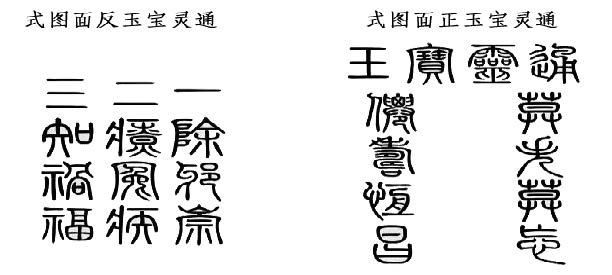
\includegraphics{1-80/8-1}

\begin{qute}

    \begin{parag}\textbf{通灵宝玉反面图式} \newline
        \indent 三二一\newline
        \indent 知疗除\newline
        \indent 祸冤邪\newline
        \indent 福疾崇\newline
    \end{parag}


    \begin{parag}
        \textbf{通灵宝玉正面图式}\newline
        \indent 仙莫\newline
        \indent 寿失\newline
        \indent 恒莫\newline
        \indent 昌忘\newline
    \end{parag}
\end{qute}


\begin{parag}
    宝钗看毕,\begin{note}甲戌双夹:余亦想见其物矣。前回中总用草蛇灰线写法,至此方细细写出,正是大关节处。\end{note}又从新翻过正面来细看,\begin{note}甲戌侧:可谓真奇之至。\end{note}口内念道:“莫失莫忘,仙寿恒昌。”\begin{note}甲戌侧:是心中沉吟,神理。甲戌眉:《石头记》立誓一笔不写一家文字。\end{note}念了两遍,乃回头向莺儿笑道:“你不去倒茶,也在这里发呆作什么?”\begin{note}甲戌双夹:请诸公掩卷合目想其神理,想其坐立之势,想宝钗面上口中。真妙!\end{note}莺儿嘻嘻笑道:“我听这两句话,倒象和姑娘的项圈上的两句话是一对儿。”\begin{note}甲戌双夹:又引出一个金项圈来,莺儿口中说出方妙。甲戌眉:恨颦儿不早来听此数语,若使彼闻之,不知又有何等妙论趣语以悦我等心臆。\end{note}宝玉听了,忙笑道:“原来姐姐那项圈上也有八个字,\begin{note}甲戌双夹:补出素日眼中虽见而实未留心。\end{note}我也鉴赏鉴赏!”宝钗道:“你别听他的话,没有什么字。”宝玉笑央:“好姐姐,你怎么瞧我的了呢。”宝钗被缠不过,因说道:“也是个人给了两句吉利话儿,所以錾上了,叫天天带著,不然,沉甸甸的有什么趣儿。”\begin{note}甲戌双夹:一句骂死天下浓妆艳饰富贵中之脂妖粉怪。\end{note}一面说,一面解了排扣,\begin{note}甲戌侧:细。\end{note}从里面大红袄上将那珠宝晶莹黄金灿烂的璎珞掏将出来。\begin{note}甲戌双夹:按,璎珞者,颈饰也!想近俗即呼为项圈者是矣。\end{note}宝玉忙托了锁看时,果然一面有四个篆字,两面八字,共成两句吉谶。亦曾按式画下形相:
\end{parag}

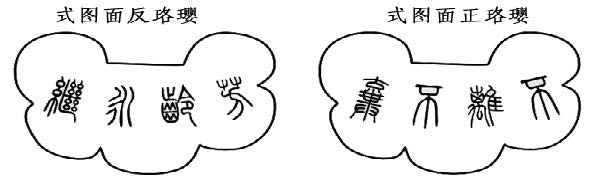
\includegraphics[]{1-80/8-2}

\begin{qute}

    \begin{parag}
        \textbf{璎珞反面式}
    \end{parag}


    \begin{parag}
        音注云:芳龄永继。\begin{note}甲戌侧:合前读之,岂非一对?\end{note}
    \end{parag}


    \begin{parag}
        \textbf{璎珞正面式}
    \end{parag}


    \begin{parag}
        音注云:不离不弃。
    \end{parag}
\end{qute}


\begin{parag}
    宝玉看了,也念了两遍,又念自己的两遍,因笑问:“姐姐这八个字倒真与我的是一对。”\begin{note}甲戌双夹:余亦谓是一对,不知干支中四注八字可与卿亦对否?甲戌眉:花看半开,酒饮微醉,此文字是也。\end{note}莺儿笑道:“是个癞头和尚送的,他说必须錾在金器上……“\begin{note}和尚在幻境中作如此勾当,亦属多事。\end{note}宝钗不待说完,便嗔他不去倒茶,\begin{note}甲戌侧:写宝钗身份。蒙侧:云龙显影法,好看煞!\end{note}一面又问宝玉从那里来。\begin{note}甲戌侧:妙神妙理,请观者自思。\end{note}
\end{parag}


\begin{parag}
    宝玉此时与宝钗就近,只闻一阵阵凉森森甜丝丝的幽香,\begin{note}蒙侧:这方是花香袭人正意。\end{note}竟不知系何香气,遂问:“姐姐熏的是什么香?我竟从未闻见过这味儿。”\begin{note}甲戌侧:不知比“群芳髓”又何如?\end{note}宝钗笑道:“我最怕熏香,好好的衣服,熏的烟燎火气的。”\begin{note}甲戌侧:真真骂死一干浓妆艳饰鬼怪。\end{note}宝玉道:“既如此,这是什么香?”宝钗想了一想,笑道:“是了,是我早起吃了丸药的香气。”\begin{note}甲戌侧:点“冷香丸”。\end{note}宝玉笑道:“什么丸药这么好闻?好姐姐,给我一丸尝尝。”\begin{note}甲戌双夹:仍是小儿语气。究竟不知别个小儿,只宝玉如此。\end{note}宝钗笑道:“又混闹了,一个药也是混吃的?”
\end{parag}


\begin{parag}
    一语未了,忽听外面人说:“林姑娘来了。”\begin{note}甲戌侧:紧处愈紧,密不容针之文。\end{note}话犹未了,林黛玉已摇摇\begin{note}甲戌侧:二字画出身份。\end{note}的走了进来,一见了宝玉,便笑道:“嗳哟,我来的不巧了!”\begin{note}甲戌侧:奇文,我实不知颦儿心中是何丘壑。\end{note}宝玉等忙起身笑让坐,宝钗因笑道:“这话怎么说?”黛玉笑道:“早知他来,我就不来了。”宝钗道:“我更不解这意。”黛玉笑道:“要来一群都来,要不来一个也不来,今儿他来了,明儿我再来,如此间错开了来著,岂不天天有人来了?\begin{note}甲戌侧:强词夺理。\end{note}也不至于太冷落,也不至于太热闹了。\begin{note}甲戌侧:好点缀。\end{note}姐姐如何反不解这意思?”\begin{note}甲戌双夹:吾不知颦儿以何物为心为齿为口为舌,实不知胸中有何丘壑。\end{note}
\end{parag}


\begin{parag}
    宝玉因见他外面罩著大红羽缎对衿褂子,\begin{note}甲戌侧:岔开文字,避繁章法,妙极妙极!\end{note}\begin{note}蒙侧:又一转换。若无此则必有宝玉之穷究,宝钗之重复,加长无味。此等文章是《西游记》的请观世音菩萨,菩萨一到,无不扫地完结者。\end{note}因问:“下雪了么?”地下婆娘们道:“下了这半日雪珠儿了。”宝玉道:“取了我的斗篷来不曾?”黛玉便道:“是不是,我来了你就该去了。”\begin{note}甲戌侧:实不知有何丘壑。\end{note}宝玉笑道:“我多早晚说要去了?不过拿来预备著。”宝玉的奶母李嬷嬷因说道:“天又下雪,也好早晚的了,就在这里同姐姐妹妹一处顽顽罢。姨妈那里摆茶果子呢。我叫丫头去取了斗篷来,说给小幺儿们散了罢。”宝玉应允。李嬷嬷出去,命小厮们都各散去不提。
\end{parag}


\begin{parag}
    这里薛姨妈已摆了几样细茶果来留他们吃茶。\begin{note}甲戌侧:是溺爱,非势利。\end{note}宝玉因夸前日在那府里珍大嫂子的好鹅掌鸭信。\begin{note}甲戌双夹:为前日秦钟之事恐观者忘却,故忙中闲笔,重一渲染。\end{note}薛姨妈听了,忙也把自己糟的取了些来与他尝。\begin{note}甲戌侧:是溺爱,非夸富。\end{note}宝玉笑道:“这个须得就酒才好。”薛姨妈便令人去灌了最上等的酒来。\begin{note}甲戌侧:愈见溺爱。\end{note}李嬷嬷便上来道:“姨太太,酒倒罢了。”\begin{note}甲戌眉:余最恨无调教之家,任其子侄肆行哺啜,观此则知大家风范。\end{note}宝玉央道:“妈妈,我只喝一钟。”李嬷嬷道:“不中用!当著老太太、太太,那怕你吃一坛呢。想那日我眼错不见一会,不知是那一个没调教的,只图讨你的好儿,不管别人死活,给了你一口酒吃,葬送的我挨了两日骂。姨太太不知道,他性子又可恶,\begin{note}甲戌侧:补出素日。\end{note}吃了酒更弄性。有一日老太太高兴了,又尽著他吃,什么日子又不许他吃,何苦我白赔在里面。”\begin{note}甲戌侧:浪酒闲茶,原不相宜。\end{note}薛姨妈笑道:“老货,\begin{note}甲戌侧:二字如闻。\end{note}你只放心吃你的去。我也不许他吃多了。便是老太太问,有我呢。”一面令小丫鬟:“来,让你奶奶们去,也吃杯搪搪雪气。”那李嬷嬷听如此说,只得和众人去吃些酒水。这里宝玉又说:“不必温暖了,我只爱吃冷的。”薛姨妈忙道:“这可使不得,吃了冷酒,写字手打颤儿。”\begin{note}甲戌侧:酷肖。\end{note}宝钗笑道:“宝兄弟,亏你每日家杂学旁收的,\begin{note}甲戌侧:著眼。若不是宝卿说出,竟不知玉卿日就何业。甲戌眉:在宝卿口中说出玉兄学业,是作微露卸春挂之萌耳,是书勿看正面为幸。\end{note}难道就不知道酒性最热,若热吃下去,发散的就快,若冷吃下去,便凝结在内,以五脏去暖他,岂不受害?从此还不快不要吃那冷的了。”\begin{note}甲戌双夹:知命知身,识理识性,博学不杂,庶可称为佳人。可笑别小说中一首歪诗,几句淫曲,便自佳人相许,岂不丑杀?\end{note}宝玉听这话有情理,\begin{note}甲戌双夹:宝玉亦听的出有情理的话来,与前回问读书家务,并皆大奇之事。\end{note}便放下冷酒,命人暖来方饮。
\end{parag}


\begin{parag}
    黛玉磕著瓜子儿,只抿著嘴笑。\begin{note}甲戌侧:实不知其丘壑,自何处设想而来?\end{note}可巧\begin{note}甲戌侧:又用此二字。\end{note}黛玉的小丫鬟雪雁走来与黛玉送小手炉,黛玉因含笑问他:“谁叫你送来的?难为他费心,那里就冷死了我!”\begin{note}甲戌侧:吾实不知何为心,何为齿、口、舌。\end{note}雪雁道:“紫鹃\begin{note}甲戌侧:鹦哥改名也。\end{note}姐姐\begin{note}甲戌双夹:又顺笔带出一个妙名来,洗尽春花腊梅等套。\end{note}怕姑娘冷,使我送来的。”黛玉一面接了,抱在怀中,笑道:“也亏你倒听他的话。我平日和你说的,全当耳旁风,怎么他说了你就依,比圣旨还快些!”\begin{note}甲戌双夹:要知尤物方如此,莫作世俗中一味酸妒狮吼辈看去。\end{note}宝玉听这话,知是黛玉借此奚落他,也无回复之词,只嘻嘻的笑两阵罢了。\begin{note}甲戌侧:这才好,这才是宝玉。\end{note}宝钗素知黛玉是如此惯了的,也不去睬他。\begin{note}甲戌侧:浑厚天成,这才是宝钗。\end{note}薛姨妈因道:“你素日身子弱,禁不得冷的,他们记挂著你倒不好?”黛玉笑道:“姨妈不知道。幸亏是姨妈这里,倘或在别人家,人家岂不恼?好说就看的人家连个手炉也没有,巴巴的从家里送个来。不说丫鬟们太小心过余,还只当我素日是这等轻狂惯了呢。”\begin{note}甲戌双夹:用此一解,真可拍案叫绝,足见其以兰为心,以玉为骨,以莲为舌,以冰为神。真真绝倒天下之裙钗矣。\end{note}\begin{note}甲戌墨笔眉\begin{subnote}似非脂批,可查看影印本\end{subnote}:强词夺理,偏他说得如许,真冰雪聪明也\end{note}薛姨妈道:“你这个多心的,有这样想,我就没这样心。”
\end{parag}


\begin{parag}
    说话时,宝玉已是三杯过去。李嬷嬷又上来拦阻。宝玉正在心甜意洽之时,和宝黛姊妹说说笑笑的,\begin{note}甲戌双夹:试问石兄:比当日青埂峰猿啼虎啸之声何如?\end{note}那肯不吃。宝玉只得屈意央告:“好妈妈,我再吃两钟就不吃了。”李嬷嬷道:“你可仔细老爷今儿在家,提防问你的书!”\begin{note}甲戌侧:不入耳之言是也。甲戌双夹:不合提此话。这是李嬷嬷激醉了的,无怪乎后文。一笑。\end{note}宝玉听了这话,便心中大不自在,慢慢的放下酒,垂了头。\begin{note}甲戌双夹:画出小儿愁蹙之状,楔紧后文。\end{note}黛玉先忙的说:“别扫大家的兴!舅舅\begin{note}甲戌侧:二字指贾政也。\end{note}若叫你,只说姨妈留著呢。这个妈妈,他吃了酒,又拿我们来醒脾了!”\begin{note}甲戌侧:这方是阿颦真意对玉卿之文。\end{note}一面悄推宝玉,使他赌气,一面悄悄的咕哝说:“别理那老货,咱们只管乐咱们的。”那李嬷嬷也素知黛玉的意思,因说道:“林姐儿,\begin{note}甲戌侧:如此之称似不能通,却是老妪真心道出。\end{note}你不要助著他了。你倒劝劝他,只怕他还听些。”林黛玉冷笑道:“我为什么助他?我也不犯著劝他。你这妈妈太小心了,往常老太太又给他酒吃,如今在姨妈这里多吃一口,料也不妨事。必定姨妈这里是外人,不当在这里的也未可定。”李嬷嬷听了,又是急,又是笑,\begin{note}甲戌侧:是认不得真,是不忍认真,是爱极颦儿、疼煞颦儿之意。\end{note}说道:“真真这林姑娘,说出一句话来,比刀子还尖。这算了什么呢。”宝钗也忍不住笑著,把黛玉腮上一拧,\begin{note}甲戌侧:我也欲拧。\end{note}说道:“真真这个颦丫头的一张嘴,叫人恨又不是,喜欢又不是。”\begin{note}甲戌侧:可知余前批不谬。\end{note}薛姨妈一面又说:“别怕,别怕,\begin{note}甲戌侧:是接前老爷问书之语。\end{note}我的儿!来这里没好的你吃,别把这点子东西唬的存在心里,倒叫我不安。只管放心吃,都有我呢。越发吃了晚饭去,便醉了,就跟著我睡罢。”因命:“再烫热酒来!姨妈陪你吃两杯,可就吃饭罢。”\begin{note}甲戌侧:二语不失长上之体,且收拾若干文,千斤力量。\end{note}宝玉听了,方又鼓起兴来。
\end{parag}


\begin{parag}
    李嬷嬷因吩咐小丫头子们:“你们在这里小心著,我家里换了衣服就来,悄悄的回姨太太,别由著他,多给他吃。”说著便家去了。这里虽还有三两个婆子,都是不关痛痒的,\begin{note}甲戌侧:写得到。\end{note}见李嬷嬷走了,也都悄悄去寻方便去了。只剩了两个小丫头子,乐得讨宝玉的欢喜。幸而薛姨妈千哄万哄的,只容他吃了几杯,就忙收过了。作酸笋鸡皮汤,宝玉痛喝了两碗,吃了半碗饭碧粳粥。\begin{note}甲戌侧:美粥名。\end{note}一时薛、林二人也吃完了饭,又酽酽的沏上茶来大家吃了。薛姨妈方放了心。雪雁等三四个丫头已吃了饭,进来伺候。黛玉因问宝玉道:“你走不走?”\begin{note}甲戌侧:妙问。\end{note}宝玉乜斜倦眼\begin{note}甲戌侧:醉意。\end{note}道:“你要走,我和你一同走。”\begin{note}甲戌侧:妙答。此等话,阿颦心中最乐。\end{note}黛玉听说,遂起身道:“咱们来了这一日,也该回去了。还不知那边怎么找咱们呢。”说著,二人便告辞。
\end{parag}


\begin{parag}
    小丫头忙捧过斗笠来,\begin{note}甲戌侧:不漏。\end{note}宝玉便把头略低一低,命他戴上。那丫头便将著大红毡斗笠一抖,才往宝玉头上一合,宝玉便说:“罢,罢!好蠢东西,你也轻些儿!难道没见过别人\begin{note}甲戌侧:“别人”者,袭人、晴雯之辈也。\end{note}戴过的?让我自己戴罢。”黛玉站在炕沿上道:“罗唆什么,过来,我瞧瞧罢。”宝玉忙就近前来。黛玉用手整理,轻轻笼住束发冠,将笠沿掖在抹额之上,将那一颗核桃大的绛绒簪缨扶起,颤巍巍露于笠外。整理已毕,端相了端相,说道:“好了,披上斗篷罢。”\begin{note}甲戌双夹:若使宝钗整理,颦卿又不知有多少文章。\end{note}\begin{note}蒙侧:知己最难逢,相逢意相同。花新水上香,花下水含红。\end{note}宝玉听了,方接了斗篷披上。薛姨妈忙道:“跟你们的妈妈都还没来呢,且略等等不迟。”宝玉道:“我们倒去等他们,有丫头们跟著也够了。”薛姨妈不放心,到底命两个妇女跟随他兄妹方罢。他二人道了扰,一径回至贾母房中。
\end{parag}


\begin{parag}
    贾母尚未用晚饭,知是薛姨妈处来,更加喜欢。\begin{note}甲戌侧:收得好极,正是写薛家母女。\end{note}因见宝玉吃了酒,遂命他自回房去歇著,不许再出来了。因命人好生看侍著。忽想起跟宝玉的人来,遂问众人:“李奶子怎么不见?”\begin{note}甲戌侧:细。\end{note}众人不敢直说家去了,\begin{note}甲戌侧:有是事,大有是事。\end{note}只说:“才进来的,想有事才去了。”宝玉踉跄回头道:“他比老太太还受用呢,问他作什么!没有他只怕我还多活两日。”一面说,一面来至自己的卧室。只见笔墨在案,\begin{note}甲戌侧:如此找前文最妙,且无逗榫之迹。\end{note}晴雯先接出来,笑说道:“好,好,要我研了那些墨,早起高兴,只写了三个字,丢下笔就走了,哄的我们等了一日。\begin{note}甲戌侧:娇憨活现,余双圈不及。\end{note}快来与我写完这些墨才罢!”\begin{note}甲戌侧:补前文之未到。\end{note}宝玉忽然想起早起的事来,因笑道:“我写的那三个字在那里呢?”晴雯笑道:“这个人可醉了。你头里过那府里去,嘱咐贴在这门斗上,这会子又这么问。我生怕别人贴坏了,\begin{note}甲戌侧:全是体贴一人。\end{note}我亲自爬高上梯的贴上,\begin{note}甲戌侧:可见可见。\end{note}这会子还冻的手僵冷的呢。”\begin{note}甲戌侧:可见可见。\end{note}\begin{note}甲戌双夹:写晴雯,是晴雯走下来,断断不是袭人、平儿、莺儿等语气。\end{note}宝玉听了,笑\begin{note}甲戌侧:是醉笑。\end{note}道:“我忘了。你的手冷,我替你渥著。”说著便伸手携了晴雯的手,同仰首看门斗上新书的三个字。\begin{note}甲戌侧:究竟不知是三个什么字,妙!\end{note}\begin{note}甲戌眉:誓不作开门见山文字。\end{note}
\end{parag}


\begin{parag}
    一时黛玉来了,宝玉笑道:“好妹妹,你别撒谎,你看这三个字那一个好?”黛玉仰头看里间门斗上,新贴了三个字,写著“绛芸轩”。\begin{note}甲戌侧:出题妙。原来是这三字。\end{note}黛玉笑道:“个个都好。怎么写的这们好了?明儿也与我写一个匾。”\begin{note}甲戌侧:滑贼。\end{note}宝玉嘻嘻的笑道:“又哄我呢。”说著又问:“袭人姐姐呢?”\begin{note}甲戌侧:断不可少。\end{note}晴雯向里间炕上努嘴。\begin{note}甲戌侧:画。\end{note}宝玉一看,只见袭人和衣睡著在那里。宝玉笑道:“好,太渥早了些。”\begin{note}甲戌侧:绛芸轩中事。\end{note}因又问晴雯道:“今儿我在那府里吃早饭,有一碟子豆腐皮的包子,我想著你爱吃,和珍大奶奶说了,只说我留著晚上吃,叫人送过来的,你可吃了?”晴雯道:“快别提。一送了来,我知道是我的,偏我才吃了饭,就放在那里。后来李奶奶来了看见,说:‘宝玉未必吃了,拿了给我孙子吃去罢。’他就叫人拿了家去了。”\begin{note}甲戌双夹:奶母之倚势亦是常情,奶母之昏愦亦是常情。然特于此处细写一回,与后文袭卿之酥酪遥遥一对,足见晴卿不及袭卿远矣。余谓晴有林风,袭乃钗副,真真不假。\end{note}接著茜雪捧上茶来。宝玉因让:“林妹妹吃茶。”众人笑说:“林妹妹\begin{note}甲戌侧:三字是接上文口气而来,非众人之称。醉态逼真。\end{note}早走了,还让呢。”\begin{note}甲戌眉:写颦儿去,如此章法从何设想?奇笔奇文。\end{note}
\end{parag}


\begin{parag}
    宝玉吃了半碗茶,忽又想起早起的茶来,\begin{note}甲戌双夹:偏是醉人搜寻得出细事,亦是真情。\end{note}因问茜雪道:“早起沏了一碗枫露茶,\begin{note}甲戌侧:与“千红一窟”遥映。\end{note}我说过,那茶是三四次后才出色的,这会子怎么又沏了这个来?”\begin{note}甲戌侧:所谓闲茶是也,与前浪酒一般起落。\end{note}茜雪道:“我原是留著的,那会子李奶奶来了,他要尝尝,就给他吃了。”\begin{note}甲戌侧:又是李嬷,事有凑巧,如此类是。\end{note}宝玉听了,将手中的茶杯只顺手\begin{note}甲戌侧:是醉后,故用二字,非有心动气也。\end{note}往地下一掷,\begin{note}甲戌眉:按警幻情榜,宝玉系“情不情”。凡世间之无知无识,彼俱有一痴情去体贴。今加“大醉”二字于石兄,是因问包子、问茶、顺手掷杯、问茜雪、撵李嬷,乃一部中未有第二次事也。袭人数语,无言而止,石兄真大醉也。甲戌眉:余亦云实实大醉也。难辞醉闹,非薛蟠纨绔辈可比!\end{note}豁啷一声,打了个粉碎,泼了茜雪一裙子的茶。又跳起来问著茜雪道:“他是你那一门子的奶奶,你们这么孝敬他?不过是仗著我小时候吃过他几日奶罢了。\begin{note}甲戌侧:真醉了。\end{note}如今逞的他比祖宗还大了。如今我又吃不著奶了,白白的养著祖宗作什么!撵了出去,大家干净!”\begin{note}甲戌侧:真真大醉了。\end{note}说著便要去立刻回贾母,撵他乳母。
\end{parag}


\begin{parag}
    原来袭人实未睡著,不过故意装睡,引宝玉来怄他顽耍。先闻得说字问包子等事,也还可不必起来,后来摔了茶钟,动了气,遂连忙起来解释劝阻。早有贾母遣人来问是怎么了。\begin{note}甲戌侧:断不可少之文。\end{note}袭人忙道:“我才倒茶来,被雪滑倒了,\begin{note}甲戌侧:现成之至,瞧他写袭卿为人。\end{note}失手砸了钟子。”一面又安慰宝玉道:“你立意要撵他也好,\begin{note}甲戌侧:二字奇,使人一惊。\end{note}我们也都愿意出去,不如趁势连我们一齐撵了,我们也好,你也不愁再有好的来伏侍你。”宝玉听了这话,方无了言语,被袭人等扶至炕上,脱换了衣服。不知宝玉口内还说些什么,只觉口齿缠绵,眼眉愈加饧涩,\begin{note}甲戌侧:二字带出平素形象。\end{note}忙伏侍他睡下。袭人伸手从他项上摘下那通灵玉来,用自己的手帕包好,塞在褥下,次日带时便冰不著脖子。\begin{note}甲戌双夹:试问石兄:此一渥,比青埂峰下松风明月如何?\end{note}那宝玉就枕便睡著了。彼时李嬷嬷等已进来了,听见醉了,不敢前来再加触犯,只悄悄的打听睡了,方放心散去。\begin{note}甲戌侧:交代清楚。“塞玉”一段,又为“误窃”一回伏线。晴雯茜雪二婢又为后文先作一引。甲戌眉:偷度金针法,最巧。\end{note}
\end{parag}


\begin{parag}
    次日醒来,\begin{note}甲戌双夹:以上已完正题,以下是后文引子,前文之余波。此文收法与前数回不同矣。\end{note}就有人回:“那边小蓉大爷带了秦相公来拜。”宝玉忙接了出去,领了拜见贾母。贾母见秦钟形容标致,举止温柔,堪陪宝玉读书,\begin{note}甲戌侧:娇养如此,溺爱如此。\end{note}心中十分欢喜,便留茶留饭,又命人带去见王夫人等。众人因素爱秦氏,今见了秦钟是这般人品,也都欢喜,临去时都有表礼。贾母又与了一个荷包并一个金魁星,\begin{note}甲戌眉:作者今尚记金魁星之事乎?抚今思昔,肠断心摧。\end{note}取“文星和合”之意。又嘱咐他道:“你家住的远,或有一时寒热饥饱不便,只管住在这里,不必限定了。只和你宝叔在一处,别跟著那些不长进的东西们学。”\begin{note}甲戌侧:总伏后文。\end{note}秦钟一一的答应,回去禀知。
\end{parag}


\begin{parag}
    他父亲秦业\begin{note}甲戌双夹:妙名。业者,孽也,盖云情因孽而生也。\end{note}现任营缮郎,\begin{note}甲戌双夹:官职更妙,设云因情孽而缮此一书之意。\end{note}年近七十,夫人早亡。因当年无儿女,便向养生堂抱了一个儿子并一个女儿。谁知儿子又死了,\begin{note}甲戌侧:一顿。\end{note}只剩女儿,小名唤可儿,\begin{note}甲戌双夹:出明秦氏究竟不知系出何氏,所谓寓褒贬、别善恶是也。秉刀斧之笔、具菩萨之心亦甚难矣,如此写出可儿来历亦甚苦矣。又知作者是欲天下人共来哭此情字。甲戌眉:写可儿出身自养生堂,是褒中贬。后死封龙禁尉,是贬中褒。灵巧一至于此。\end{note}长大时,生的形容袅娜,性格风流。\begin{note}甲戌侧:四字便有隐意。《春秋》字法。\end{note}因素与贾家有些瓜葛,故结了亲,许与贾蓉为妻。那秦业至五旬之上方得了秦钟。因去岁业师亡故,未暇延请高明之士,只得暂时在家温习旧课。正思要和亲家\begin{note}甲戌侧:指贾珍。\end{note}去商议送往他家塾中,暂且不致荒废,可巧遇见了宝玉这个机会。又知贾家塾中现今司塾的是贾代儒,\begin{note}甲戌侧:随笔命名,省事。\end{note}乃当今之老儒,秦钟此去,学业料必进益,成名可望,因此十分喜悦。只是宦囊羞涩,那贾家上上下下都是一双富贵眼睛,\begin{note}甲戌侧:为天下读书人一哭、寒素人一哭。\end{note}容易拿不出来,又恐误了儿子的终身大事,\begin{note}甲戌侧:原来读书是终生大事。\end{note}说不得东拼西凑的恭恭敬敬\begin{note}甲戌侧:四字可思,近之鄙薄师傅者来看。\end{note}封了二十四两贽见礼,\begin{note}甲戌双夹:可知“宦囊羞涩”与“东拼西凑”等样,是特为近日守钱虏而不使子弟读书之辈一大哭。\end{note}亲自带了秦钟,来代儒家拜见了。然后听宝玉上学之日,好一同入塾。\begin{note}甲戌双夹:不想浪酒闲茶一段金玉旖旎之文后,忽用此等寒瘦古拙之词收住,亦行文之大变体处。《石头记》多用此法,历观后文便知。\end{note}正是:
\end{parag}


\begin{poem}
    \begin{pl}早知日后闲争气,岂肯今朝错读书。\end{pl}
    \begin{note}甲戌侧:这是隐语微词,岂独此指一事哉?余则谓读书正为争气。但此“争气”与彼“争气”不同。写来一笑。\end{note}
\end{poem}